\documentclass[10pt,a4paper,UTF8]{ctexart}
\usepackage{geometry}%用于设置上下左右页边距
	\geometry{left=2.5cm,right=2.5cm,top=3.2cm,bottom=2.8cm}
\usepackage{xeCJK,amsmath,paralist,enumerate,booktabs,multirow,graphicx,subfig,setspace,listings,lastpage,hyperref}
\usepackage{amsthm, amssymb, bm, color, framed, graphicx, hyperref, mathrsfs}
\usepackage{mathrsfs}  
	\setlength{\parindent}{2em}
	\lstset{language=Matlab}%
\usepackage{fancyhdr}
\usepackage{graphicx}
\usepackage{listings}
\usepackage{xcolor}
\usepackage{float}

\definecolor{mKeyword}{RGB}{0,0,255}          % bule
\definecolor{mString}{RGB}{160,32,240}        % purple
\definecolor{mComment}{RGB}{34,139,34}        % green
\definecolor{mNumber}{RGB}{128,128,128} 

\lstdefinestyle {njulisting} {
	basewidth = 0.5 em,
	lineskip = 3 pt,
	basicstyle = \small\ttfamily,
	% keywordstyle = \bfseries,
	commentstyle = \itshape\color{gray}, 
	basicstyle=\small\ttfamily,
	keywordstyle={\color{mKeyword}},     % sets color for keywords
	stringstyle={\color{mString}},       % sets color for strings
	commentstyle={\color{mComment}},     % sets color for comments
	numberstyle=\tiny\color{mNumber},
	numbers = left,
	captionpos = t,
	breaklines = true,
	xleftmargin = 2 em,
	xrightmargin = 2 em,
	frame=tlrb
}

\lstset{
style = njulisting, % 调用上述样式 
flexiblecolumns % 允许调整字符宽度
}

\pagestyle{fancy}
\lhead{\textsc{Foundation of Computing System}}
\rhead{\textsc{Nanjing University}}
\cfoot{\thepage}
\renewcommand{\headrulewidth}{0.4pt}
\renewcommand{\theenumi}{(\arabic{enumi})}


\definecolor{shadecolor}{RGB}{241, 241, 255}

\newcommand{\problemname}{待定义}
\newenvironment{problem}{\begin{shaded}\par\noindent\textbf{题目\  \problemname}}{\end{shaded}\par}
\newenvironment{solution}{\par\noindent\textbf{解答}\ }{\par}
\newenvironment{note}{\par\noindent\textbf{题目 \problemname 的注记}}{\par}

\begin{document}

\begin{center}
\LARGE\textbf{第十章习题参考答案}
\end{center}

{\kaishu 包含题目:习题$10.1$和$10.2$}


% \begin{figure}[H]
% 	\centering
% 	\includegraphics[scale=0.3]{img/}
% \end{figure}

% \lstset{language=C}
% 	\begin{lstlisting}
	
% 	\end{lstlisting}



\renewcommand{\problemname}{10.1}
\begin{problem}
	下表中的DLX程序实现了什么?
\end{problem}

\begin{figure}[H]
	\centering
	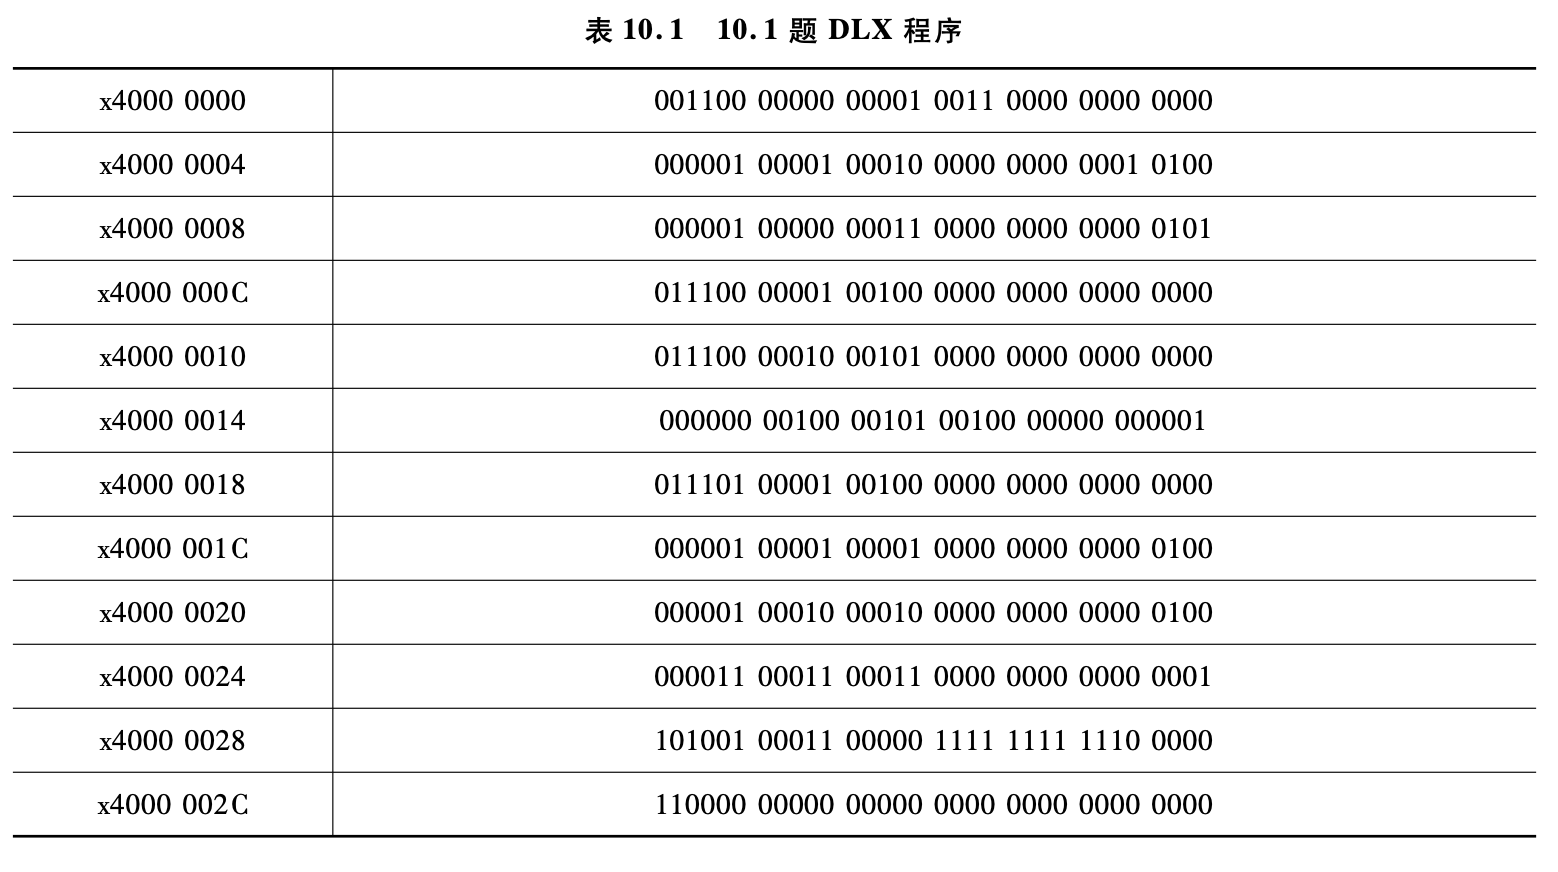
\includegraphics[scale=0.5]{img/10.1}
\end{figure}

\begin{solution}
	将机器语言指令翻译成汇编代码如下
	\begin{lstlisting}
LHI  R1, 0x3000       
ADDI  R2, R1, 0x14     
ADDI  R3, R0, 0x5     
LW  R4, R1            
LW  R5, R2           
ADD  R4, R5, R4
SW  R4, R1
ADDI  R1, R1, 0x4
ADDI  R2, R2, 0x4
SUBI  R3, R3, 0x1
BNEZ  R3, 0xFEE0
TRAP  #0
	\end{lstlisting}
	
	该段程序的作用是将0x3000 0000 到 0x 3000 0013 存储的5个整数分别与存储在0x3000 0014
	到0x3000 0028的5个整数分别相加,并将结果写入到前者对应的地址。
\end{solution}


\renewcommand{\problemname}{10.2}
\begin{problem}
	对于下表所示的机器语言程序,R1的初始值是什么时,可以使得R2的最终值为7?
\end{problem}

\begin{figure}[H]
	\centering
	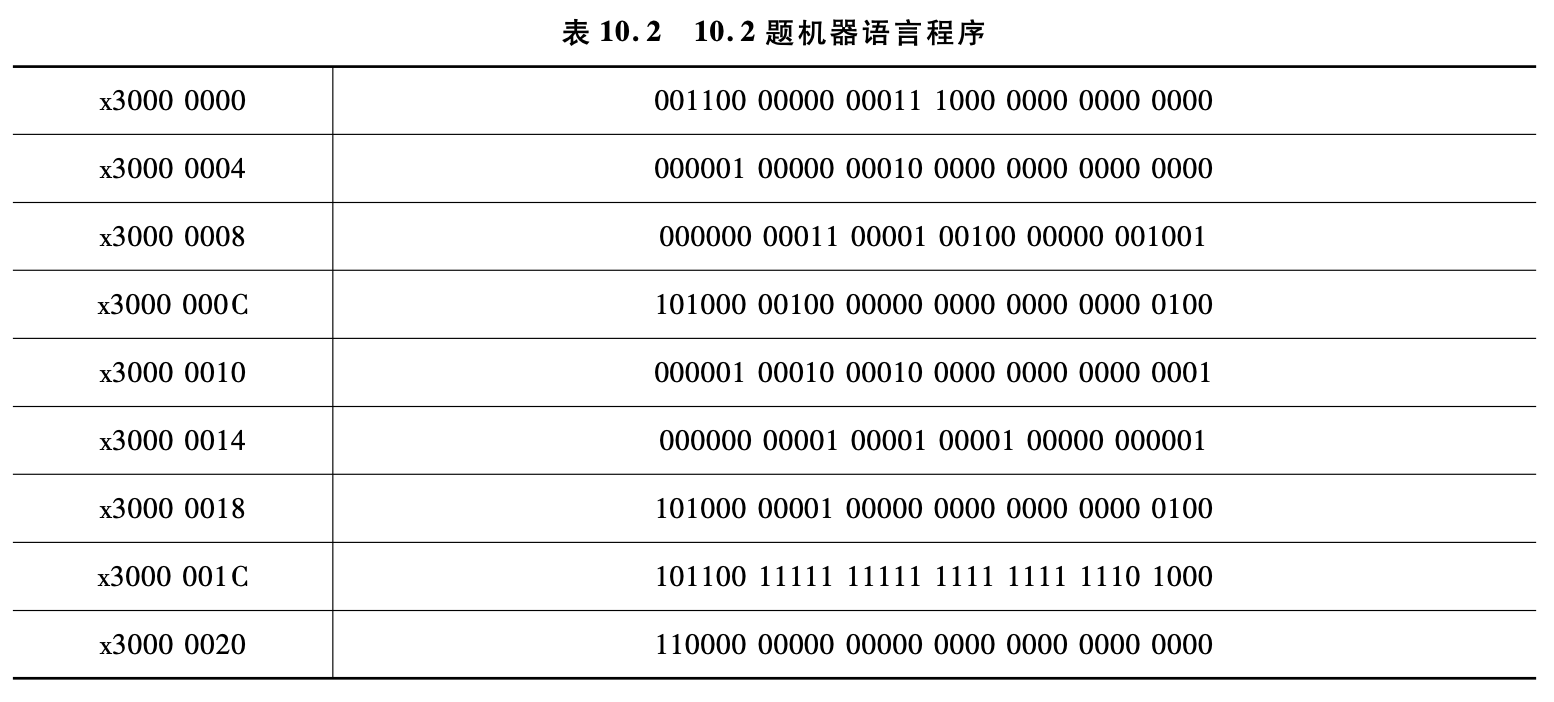
\includegraphics[scale=0.5]{img/10.2}
\end{figure}

\begin{solution}
	将机器语言指令翻译成汇编代码如下
	\begin{lstlisting}
LHI  R3, R0, 0x8000
ADDI  R2, R0, 0x0
AND  R4, R3, R1
BEQZ  R4, 0x4
ADDI  R2, R2, 0x1
ADD  R1, R1, R1
BEQZ  R1, 0x4
J  0xFFFE8
TRAP  #0	
	\end{lstlisting}

	当R1的内容为0xFE00 0000时,R2的最终值为7。
\end{solution}

\end{document}
